% !TeX spellcheck = es_MX-SpanishMexico
%----------------------------------------------------------------------------------------------------
%                           		  ENTRE LÍNEAS DE TIERRA

% Curso: Arqueología Bíblica
% Módulo 1: Introducción, Definiciones y Conceptos
% Elabora: Rodrigo Gerardo Trejo Arriaga

%----------------------------------------------------------------------------------------------------

% FORMATO DEL DOCUMENTO


\documentclass[11pt]{article} % Letra estandar

\usepackage[utf8]{inputenc}

%\usepackage{tgadventor}
%\renewcommand{\familydefault}{\sfdefault}

\usepackage[light,math]{iwona}

\usepackage[T1]{fontenc}


\usepackage[spanish]{babel}
\addto\captionsspanish{\renewcommand{\abstractname}{\large{Introducción}}}

\usepackage[margin=1in,letterpaper]{geometry}

\usepackage{fancyhdr} % Paquete para personalizar encabezado y pie de página
\pagestyle{fancy} % Establece que personalizaremos el pie de pagina y el encabezado
\setlength{\headheight}{13.59999pt} % Establece la altura del encabezado
\fancyhead[R]{\textcolor{darkBlue}{Teoría de la Computación}} % Encabezado derecho
\fancyhead[L]{\textit{\textcolor{darkBlue}{Escuela Superior de Cómputo}}} % Encabezado izquierdo
\fancyfoot[L]{\textit{\textcolor{darkBlue}{Práctica 9}}} % Pie de página izquierdo 
\fancyfoot[R]{\textcolor{darkBlue}{\thepage}} % Pie de página  derecho
\fancyfoot[C]{} % Elimina la nueración central de páginas en el pie de página
\renewcommand{\headrulewidth}{0.5pt} % Grosor de la linea de encabezado
\renewcommand{\footrulewidth}{0.5pt} % Grosor de la linea de pie de página

\usepackage{enumitem}

\usepackage{changepage}

\usepackage{graphicx}

\usepackage{tabularx}

\setlength{\parskip}{8pt}

\usepackage{xcolor}
\definecolor{darkBlue}{rgb}{0,0,0.31}
%\definecolor{darkBlue}{rgb}{0,0,0.5}
\definecolor{munsell}{rgb}{0.0, 0.5, 0.69}
\definecolor{indigo}{rgb}{0.0, 0.25, 0.42}
\renewcommand{\footrulewidth}{2pt}
\renewcommand{\footrule}{\hbox to\headwidth{\color{darkBlue}\leaders\hrule height \footrulewidth\hfill}}

\usepackage{colortbl}

\usepackage{titlesec}
\titleformat{\section}
{\normalfont\Large\bfseries\color{darkBlue}}{\thesection.}{1em}{}

\usepackage{tabularx}

\usepackage{textcomp}

\usepackage{titling}

\usepackage{apacite}

\usepackage{amsmath}
\bibliographystyle{apacite}

%\usepackage{natbib}
%\setlength{\bibsep}{6pt}

\usepackage{setspace}

\usepackage{listings}


% Define tus propios colores en tonos de azul
\definecolor{codeblue}{rgb}{0.25,0.5,0.5}
\definecolor{backcolour}{rgb}{0.95,0.95,0.92}
\definecolor{commentblue}{rgb}{0.3,0.3,0.6}
\definecolor{keywordblue}{rgb}{0.2,0.2,0.7}
\definecolor{stringblue}{rgb}{0.15,0.2,0.9}

\lstdefinestyle{bluepythonstyle}{
	language=Python,
	basicstyle=\ttfamily\small,
	commentstyle=\color{commentblue},
	keywordstyle=\color{keywordblue},
	numberstyle=\tiny\color{codeblue},
	stringstyle=\color{stringblue},
	backgroundcolor=\color{backcolour},
	breaklines=true,
	captionpos=b,
	abovecaptionskip=1\baselineskip,
	showstringspaces=false,
	frame=lines,
	numbers=left,
	xleftmargin=\parindent,
	tabsize=4
}
\lstset{style=bluepythonstyle}



\renewcommand{\thesection}{\Roman{section}}

%----------------------------------------------------------------------------------------------------
% CUERPO DEL DOCUMENTO

\begin{document}
	
	\begin{titlepage}
		\centering
		{
\includegraphics[width=0.25\textwidth]{descarga}\par}
		\vspace{0.5cm}
		{\bfseries\huge Escuela Superior de Cómputo \par}
		\vspace{0.7cm}
		{\scshape\LARGE Teoría de la Computación \par}
		\vspace{0.3cm}
		\vspace{3.1cm}
		{\scshape \Huge \textbf{Práctica 9:}  \par}
		\vspace{0.03cm}
		{{\LARGE \textit{TURING MACHINE}} \par}
		%\vfill
		\vspace{3.5cm}
		{\Large Autor: \par}
		{\Large Rodrigo Gerardo Trejo Arriaga \par}
		%\vfill
		\vspace{3cm}
		{\Large Diciembre 2023 \par}
	\end{titlepage}
	
	\begin{center}
		\vspace*{0.1cm}
		{\huge \textcolor{darkBlue}{\textbf{Práctica 9:}} \par}
		
		{\Large \textcolor{darkBlue}{\textbf{\textit{TURING MACHINE}}}}
	\end{center}
	
	
	\section{Introducción}
	La Máquina de Turing, nombrada así por su inventor Alan Turing en 1936, es un modelo matemático fundamental en la teoría de la computación. Turing introdujo este concepto en su trabajo seminal "On Computable Numbers, with an Application to the Entscheidungsproblem", que sentó las bases para la computación moderna [1].
	
	\section{Definición de la Máquina de Turing}
	Una Máquina de Turing es un dispositivo teórico que manipula símbolos contenidos en una cinta de longitud infinita según un conjunto de reglas. Formalmente, una Máquina de Turing se define como una 7-tupla \( (Q, \Gamma, b, \Sigma, \delta, q_0, F) \) donde [1]:
	
	\begin{itemize}
		\item \( Q \) es un conjunto finito de estados.
		\item \( \Gamma \) es un conjunto finito de símbolos de la cinta, donde \( b \in \Gamma \) es el símbolo en blanco.
		\item \( \Sigma \subseteq \Gamma \setminus \{b\} \) es el conjunto de símbolos de entrada.
		\item \( \delta: Q \times \Gamma \rightarrow Q \times \Gamma \times \{L, R\} \) es la función de transición.
		\item \( q_0 \in Q \) es el estado inicial.
		\item \( F \subseteq Q \) es el conjunto de estados finales o de aceptación.
	\end{itemize}
	
	\section{Funcionamiento}
	La máquina comienza con la cinta conteniendo una cadena de símbolos del alfabeto de entrada y el resto de la cinta en blanco. La máquina opera de acuerdo con las reglas definidas por la función de transición \( \delta \), que dicta el comportamiento de la máquina en función del estado actual y el símbolo leído de la cinta [2].
	
	\section{Relevancia en la Teoría de la Computación}
	La Máquina de Turing es un modelo importante por varias razones [2]:
	
	\begin{enumerate}
		\item \textbf{Universalidad}: La Máquina de Turing es capaz de simular cualquier algoritmo computacional.
		\item \textbf{Modelo de Cómputo}: Sirve como un modelo estándar para definir lo que es computable.
		\item \textbf{Problemas indecidibles}: Turing utilizó este modelo para demostrar la existencia de problemas indecidibles, es decir, problemas que no pueden ser resueltos por ninguna máquina de Turing.
	\end{enumerate}
	
	\section{Definición de Identificadores (ID)}
	En el contexto de Máquinas de Turing (TM), un identificador (ID) es una cadena que representa el estado actual de la máquina. Se compone de tres partes: la parte izquierda de la cinta (\(\alpha\)), el estado actual (\(q\)), y la parte derecha de la cinta (\(\beta\)). Esto se denota como \(\alpha q\beta\), donde \(\alpha\beta\) es la porción de la cinta entre los símbolos no blancos más a la izquierda y más a la derecha, inclusive [3].
	
	\subsection{Comportamiento de los ID [3]}
	\begin{itemize}
		\item El estado \(q\) está inmediatamente a la izquierda del símbolo de la cinta que está siendo escaneado.
		\item Si \(q\) está al final derecho, está escaneando el símbolo blanco (\(B\)).
		\item Si \(q\) escanea un \(B\) al principio de la izquierda, entonces cualquier \(B\) consecutivo a la derecha de \(q\) forma parte de \(\alpha\).
	\end{itemize}
	
	\subsection*{Notación de Transiciones}
	Para las transiciones de la TM, podemos usar los símbolos \(\vdash\) y \(\vdash^*\) para representar "se convierte en un movimiento" y "se convierte en cero o más movimientos", respectivamente [3].
	
	\subsection*{Ejemplo}
	Un ejemplo de las movidas de una TM puede ser representado como sigue [3]:
	\[ q_0 00 \vdash 0q_0 0 \vdash 00q_0 \vdash 00q_1 \vdash^* 000q_f \]
	
	
	
	\section{Instrucciones}
	
	El objetivo de esta práctica es implementar una Máquina de Turing que reconozca el lenguaje \(\{0^n1^n | n \geq 1\}\). Este lenguaje consiste en cadenas con un número igual de ceros seguidos por unos. La especificación de la máquina se basa en el ejercicio 8.2, segunda edición, del libro de John Hopcroft.
	
	\subsection*{Requerimientos}
	\begin{enumerate}
		\item El programa debe aceptar una cadena de entrada definida por el usuario o generada automáticamente, con una longitud máxima de 1000 caracteres.
		\item La salida del programa debe ser un archivo de texto con descripciones instantáneas de cada paso de la computación de la máquina.
		\item Se debe proporcionar una animación de la Máquina de Turing para cadenas de entrada de longitud menor o igual a 16 caracteres.
	\end{enumerate}
	
	\subsection*{Tabla de Transiciones}
	La siguiente tabla representa la función de transición de la Máquina de Turing para el ejercicio mencionado.
	
	\begin{table}[h]
		\centering
		\begin{tabular}{|c|c|c|c|c|c|}
			\hline
			\textbf{State} & \textbf{0} & \textbf{1} & \textbf{X} & \textbf{Y} & \textbf{B} \\ % Aquí había un error en la cantidad de columnas.
			\hline
			\(q_0\) & \( (q_1, X, R) \) & - & - & \( (q_3, Y, R) \) & - \\
			\(q_1\) & \( (q_1, 0, R) \) & \( (q_2, Y, L) \) & - & \( (q_1, Y, R) \) & - \\
			\(q_2\) & \( (q_2, 0, L) \) & - & \( (q_0, X, R) \) & \( (q_2, Y, L) \) & - \\
			\(q_3\) & - & - & - & \( (q_3, Y, R) \) & \( (q_4, B, R) \) \\
			\(q_4\) & - & - & - & - & - \\
			\hline
		\end{tabular}
		\caption{Tabla de transiciones de la Máquina de Turing para aceptar el lenguaje \(\{0^n1^n | n \geq 1\}\).}
	\end{table}

	
	\newpage
	
	\section{Resultados}
	
	
	\begin{figure}[h]
		\centering
		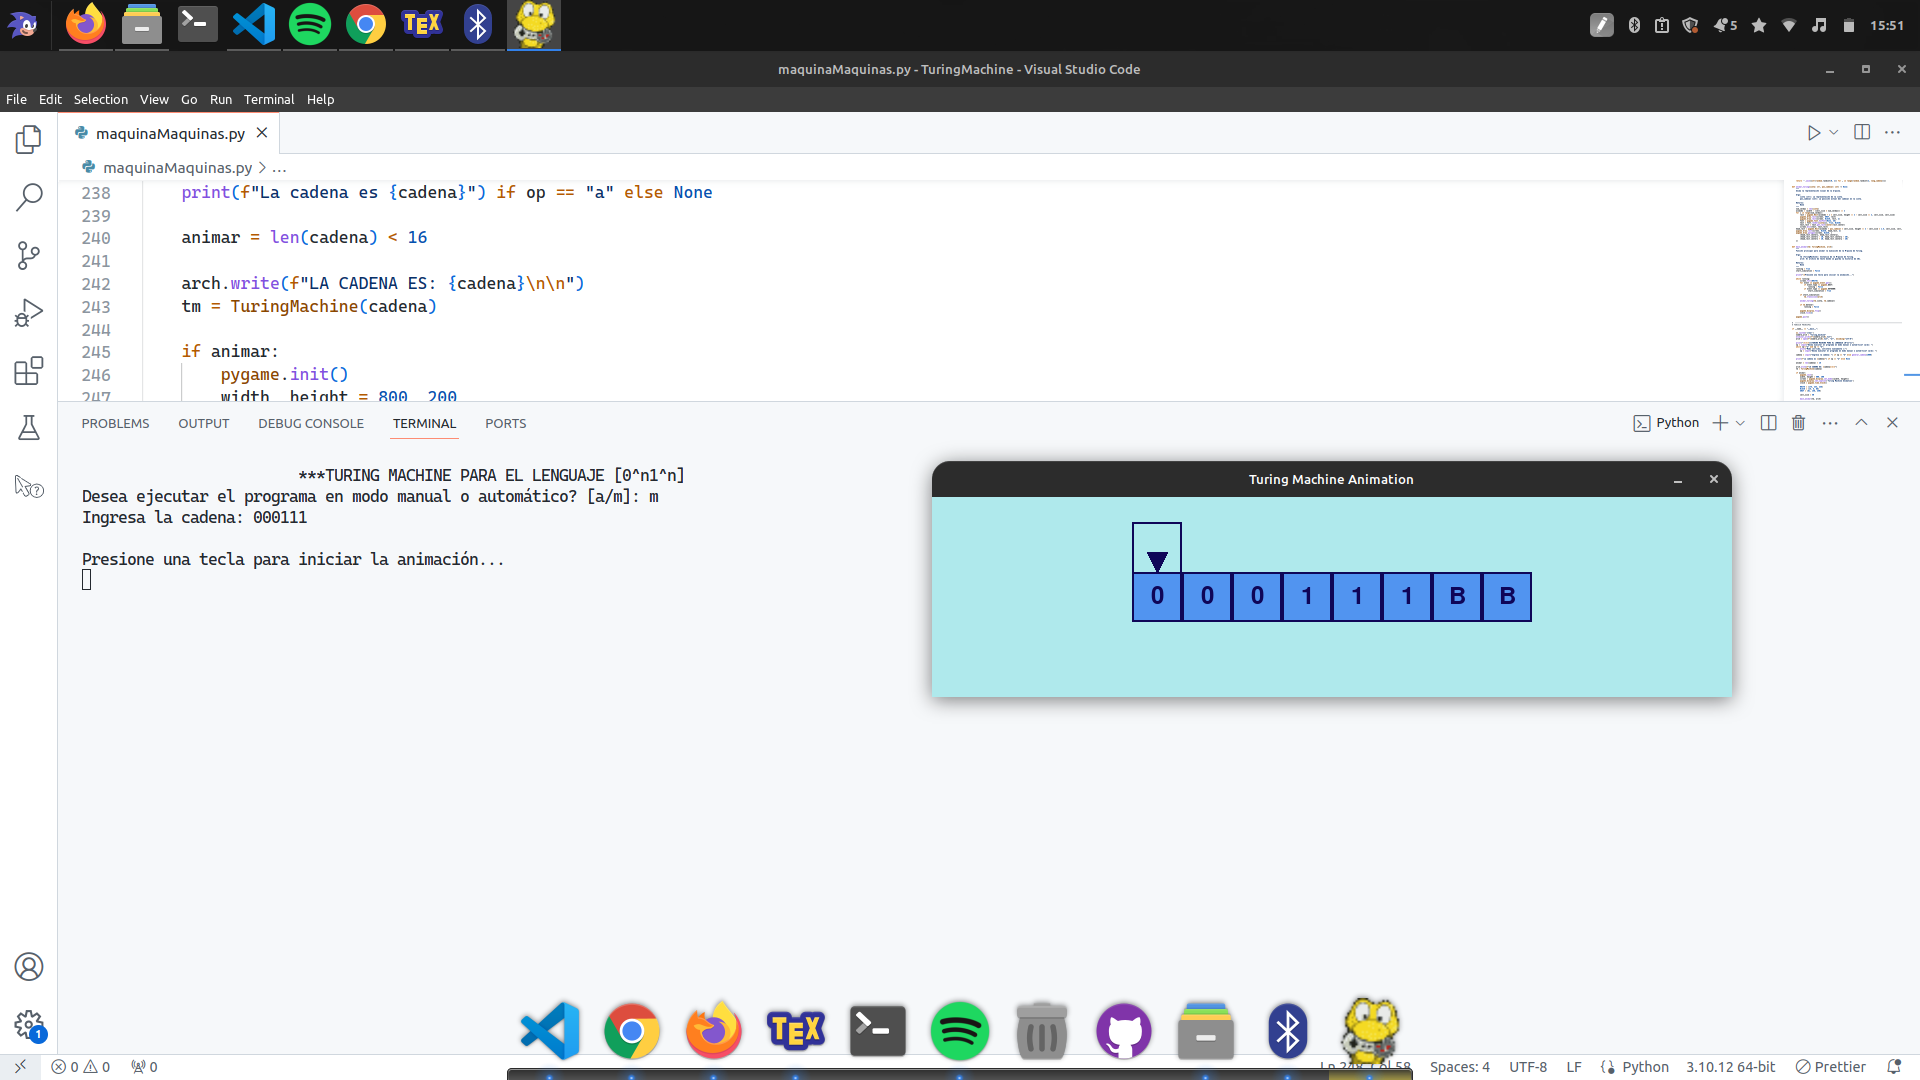
\includegraphics[width=0.8\textwidth]{manual1}
		\caption{Cadena 000111 - Animación de la Máquina de Turing}
	\end{figure}
	
	
	\begin{figure}[h]
		\centering
		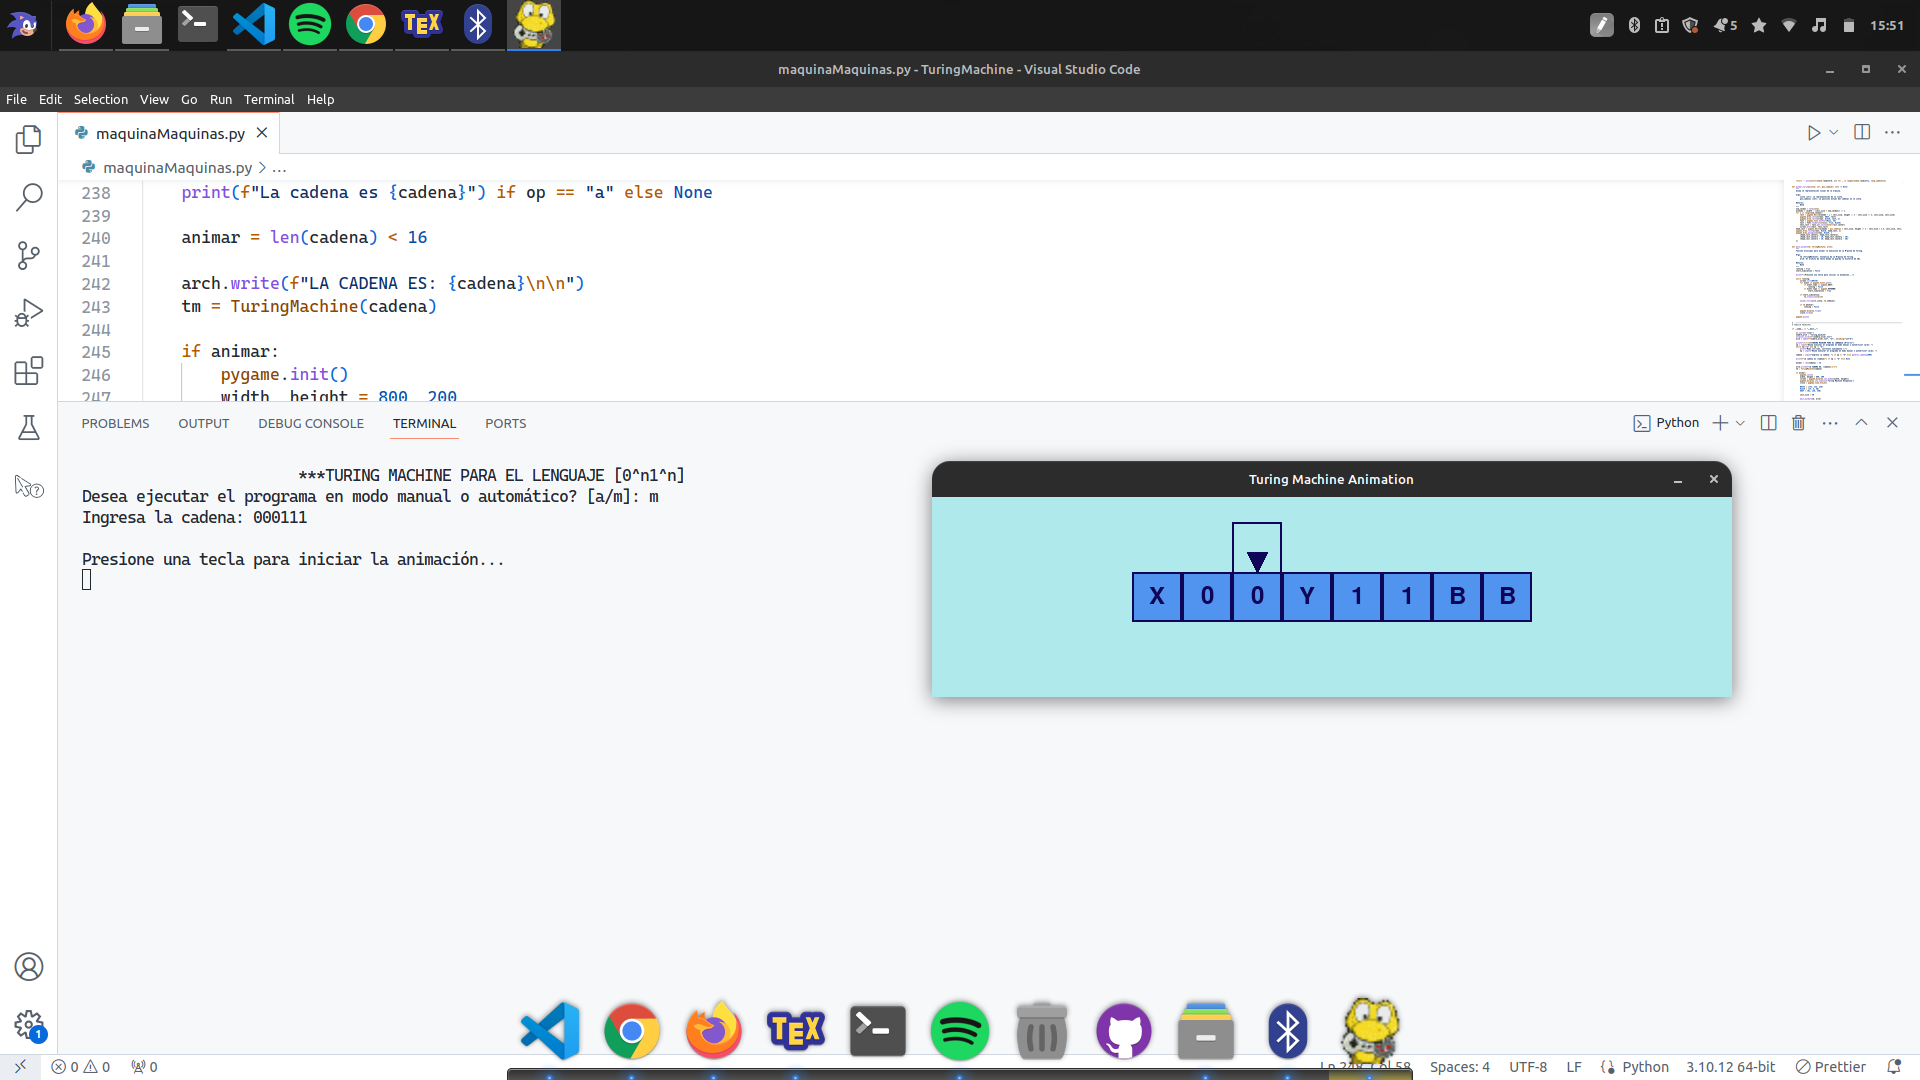
\includegraphics[width=0.8\textwidth]{manual2}
		\caption{Cadena 000111 - Animación de la Máquina de Turing}
	\end{figure}
	\newpage
	
	
	\begin{figure}[h]
		\centering
		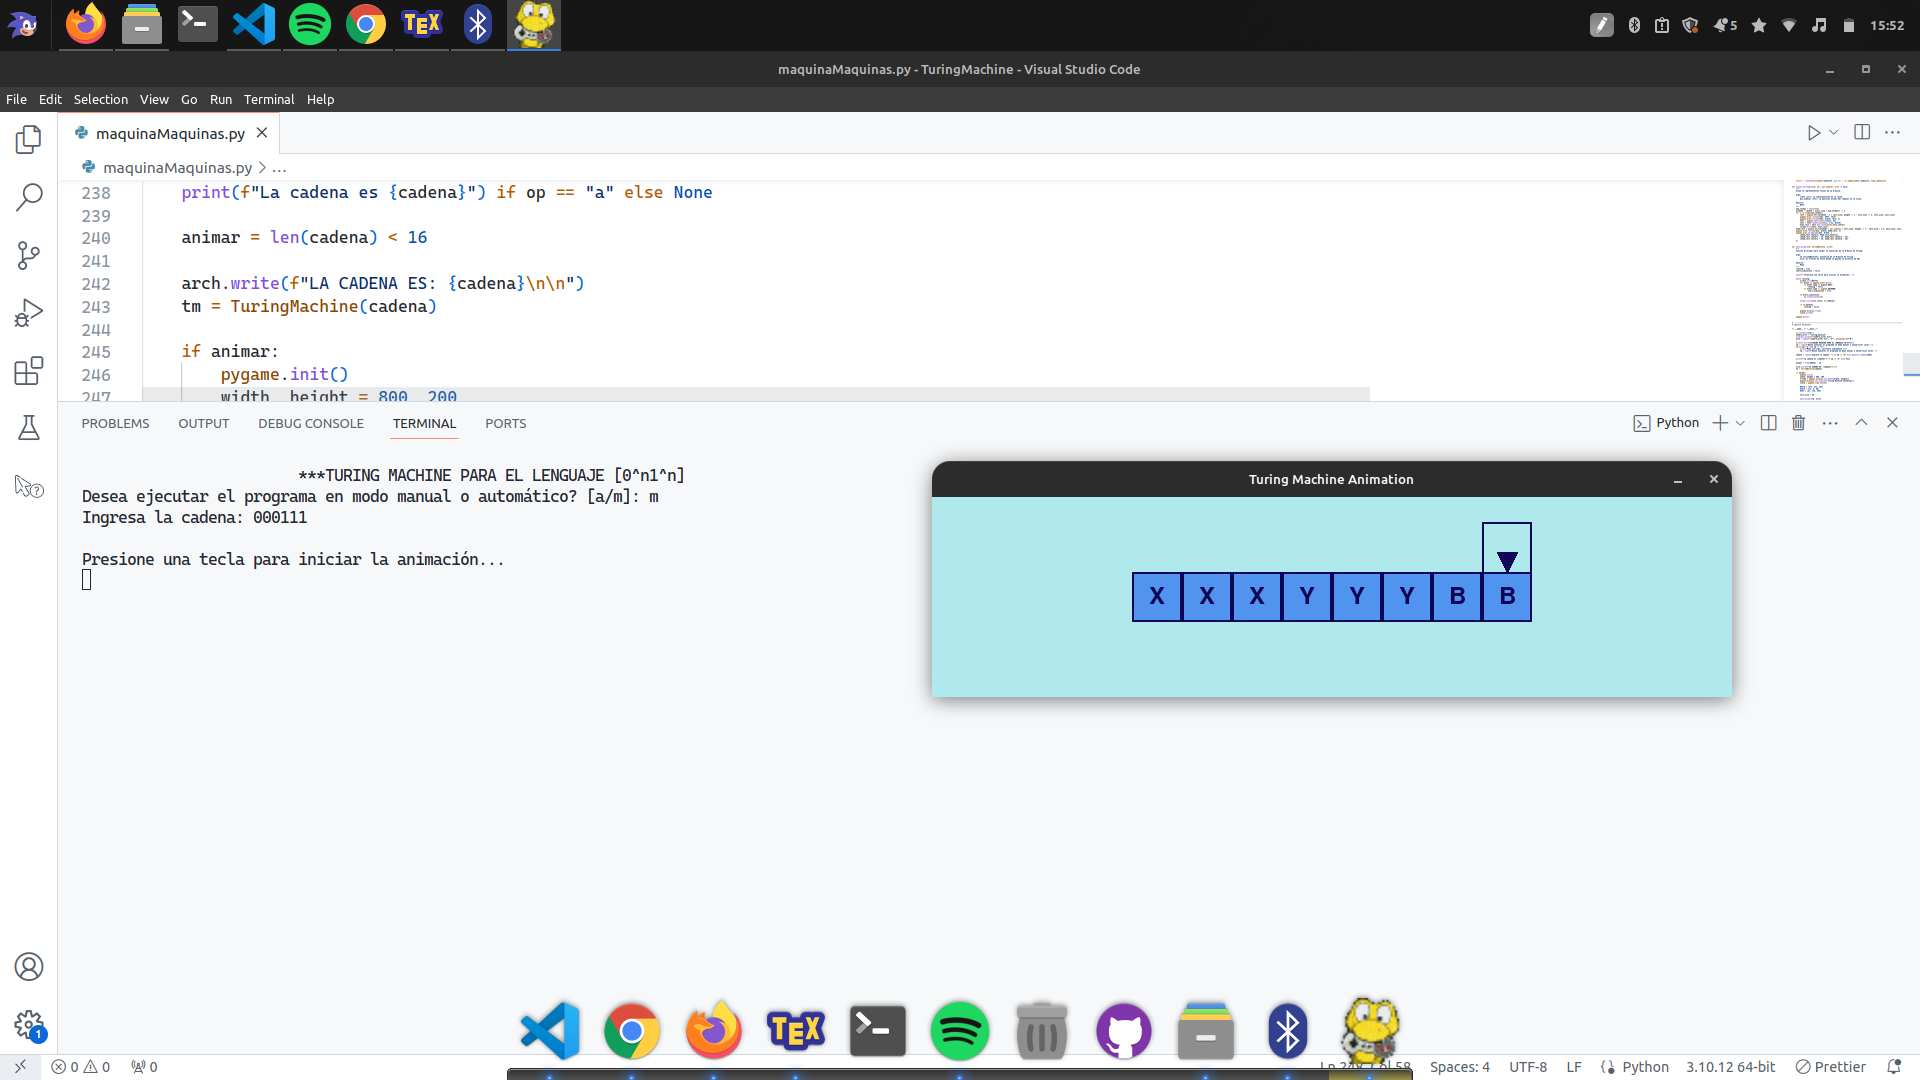
\includegraphics[width=0.8\textwidth]{manual3}
		\caption{Cadena 000111 - Animación de la Máquina de Turing}
	\end{figure}
	
	\begin{figure}[h]
		\centering
		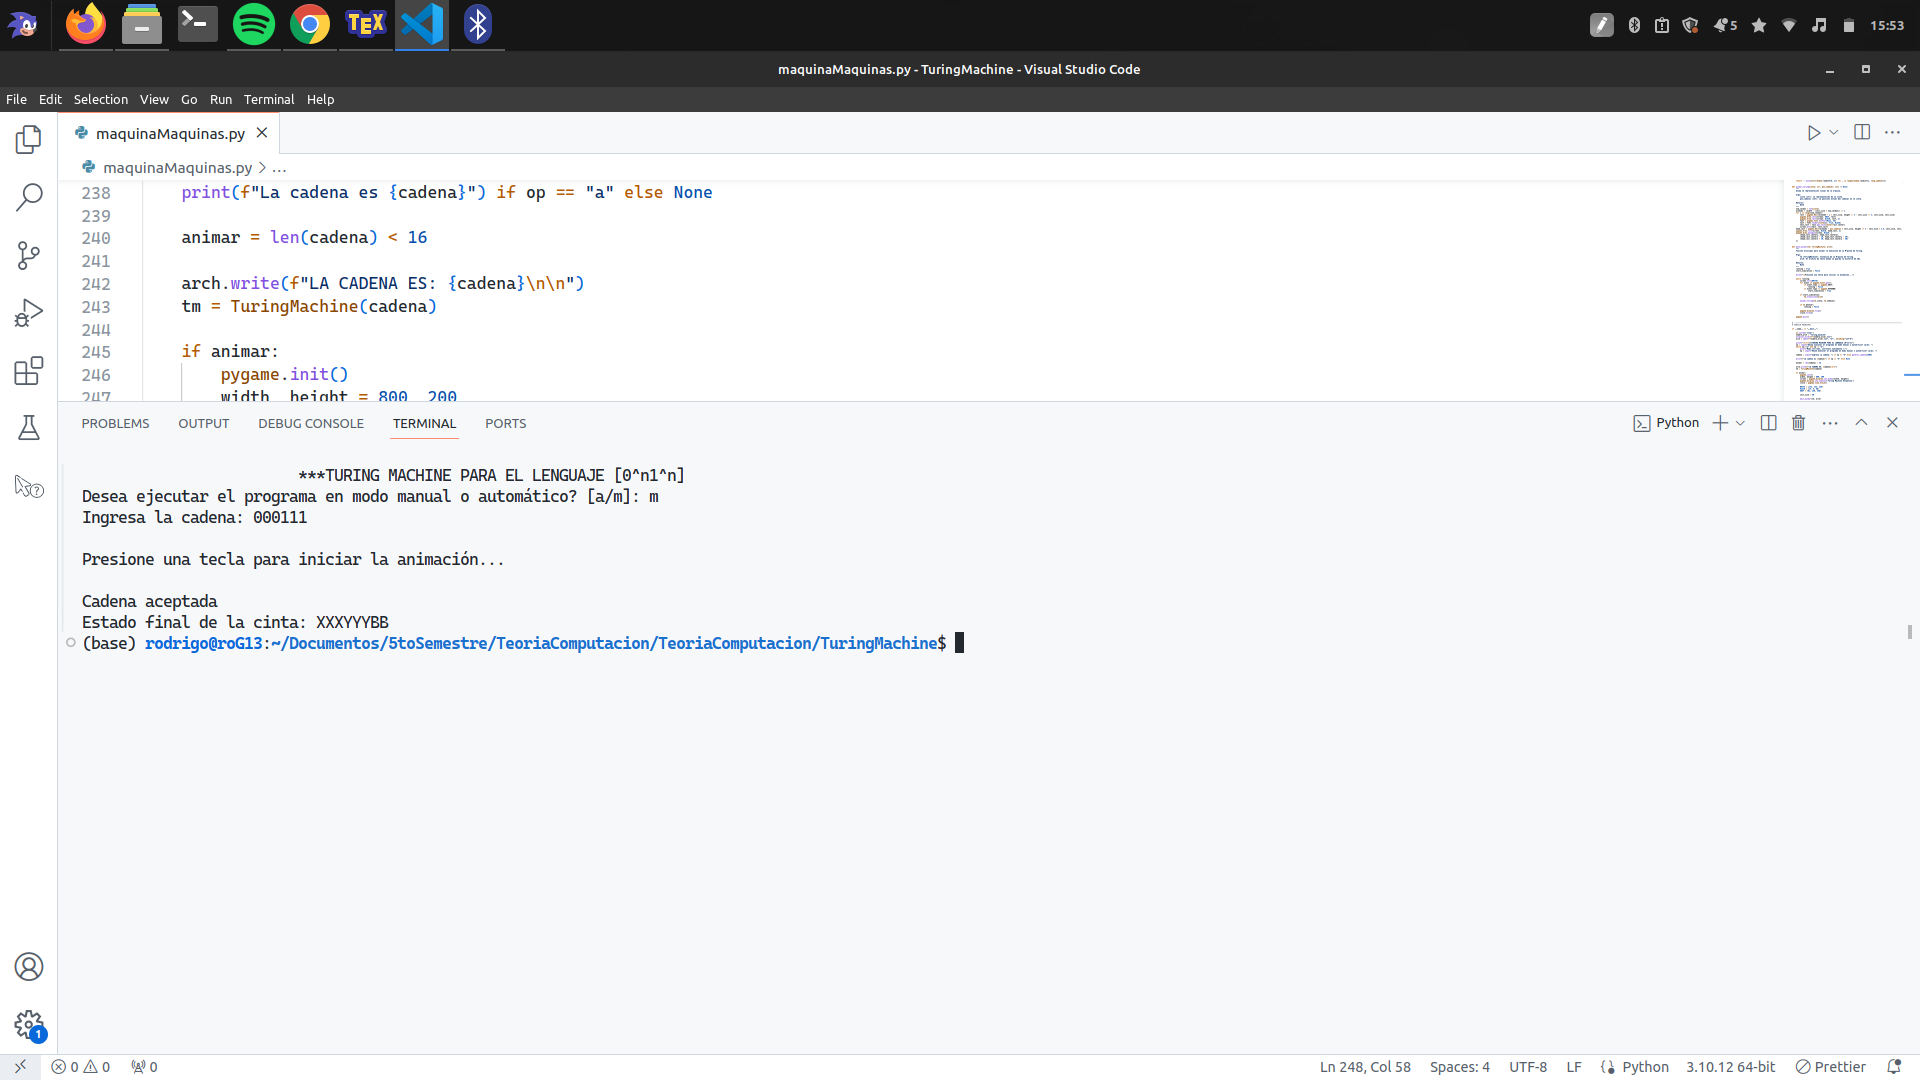
\includegraphics[width=0.8\textwidth]{manual4}
		\caption{Cadena 000111 - Resultados de la Máquina de Turing}
	\end{figure}
	
	\newpage

	
	\begin{figure}[h]
		\centering
		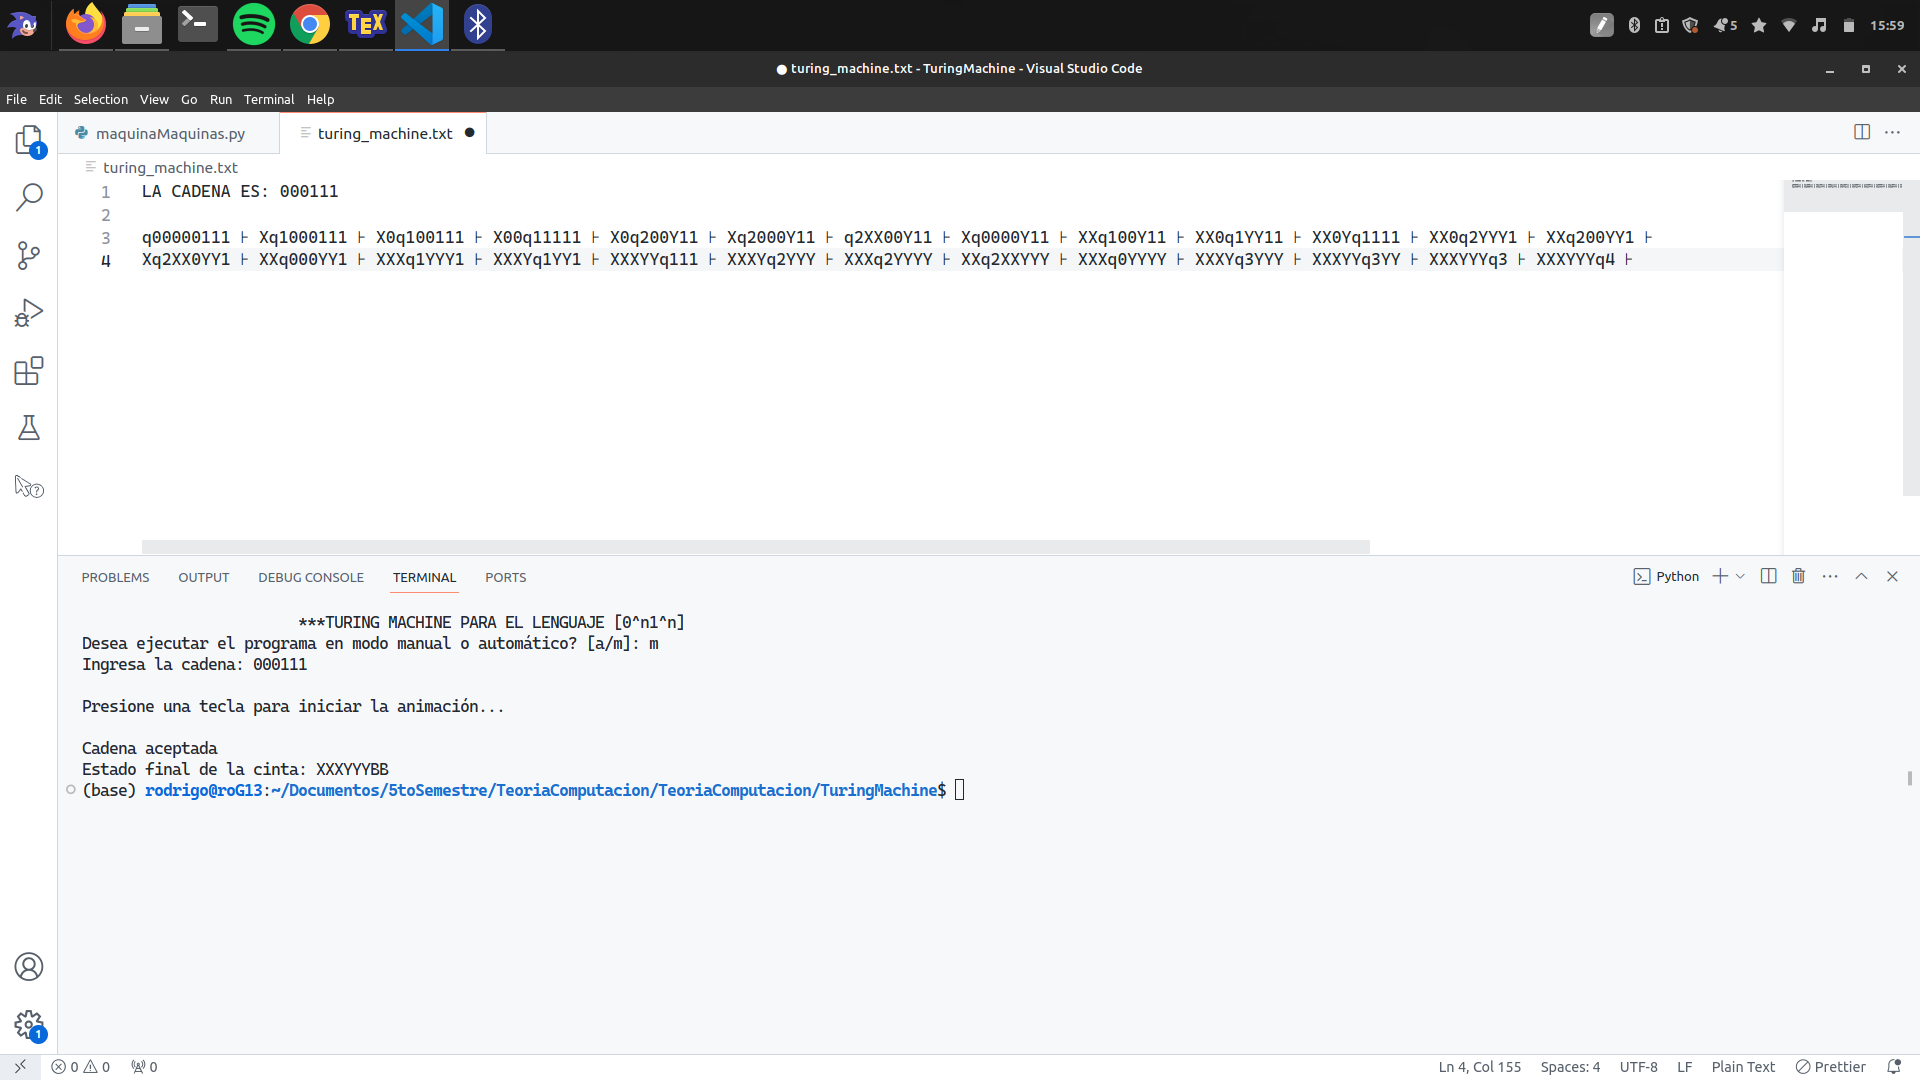
\includegraphics[width=0.8\textwidth]{arch1}
		\caption{Cadena 000111 - Archivo de los ID's}
	\end{figure}
	\begin{figure}[h]
		\centering
		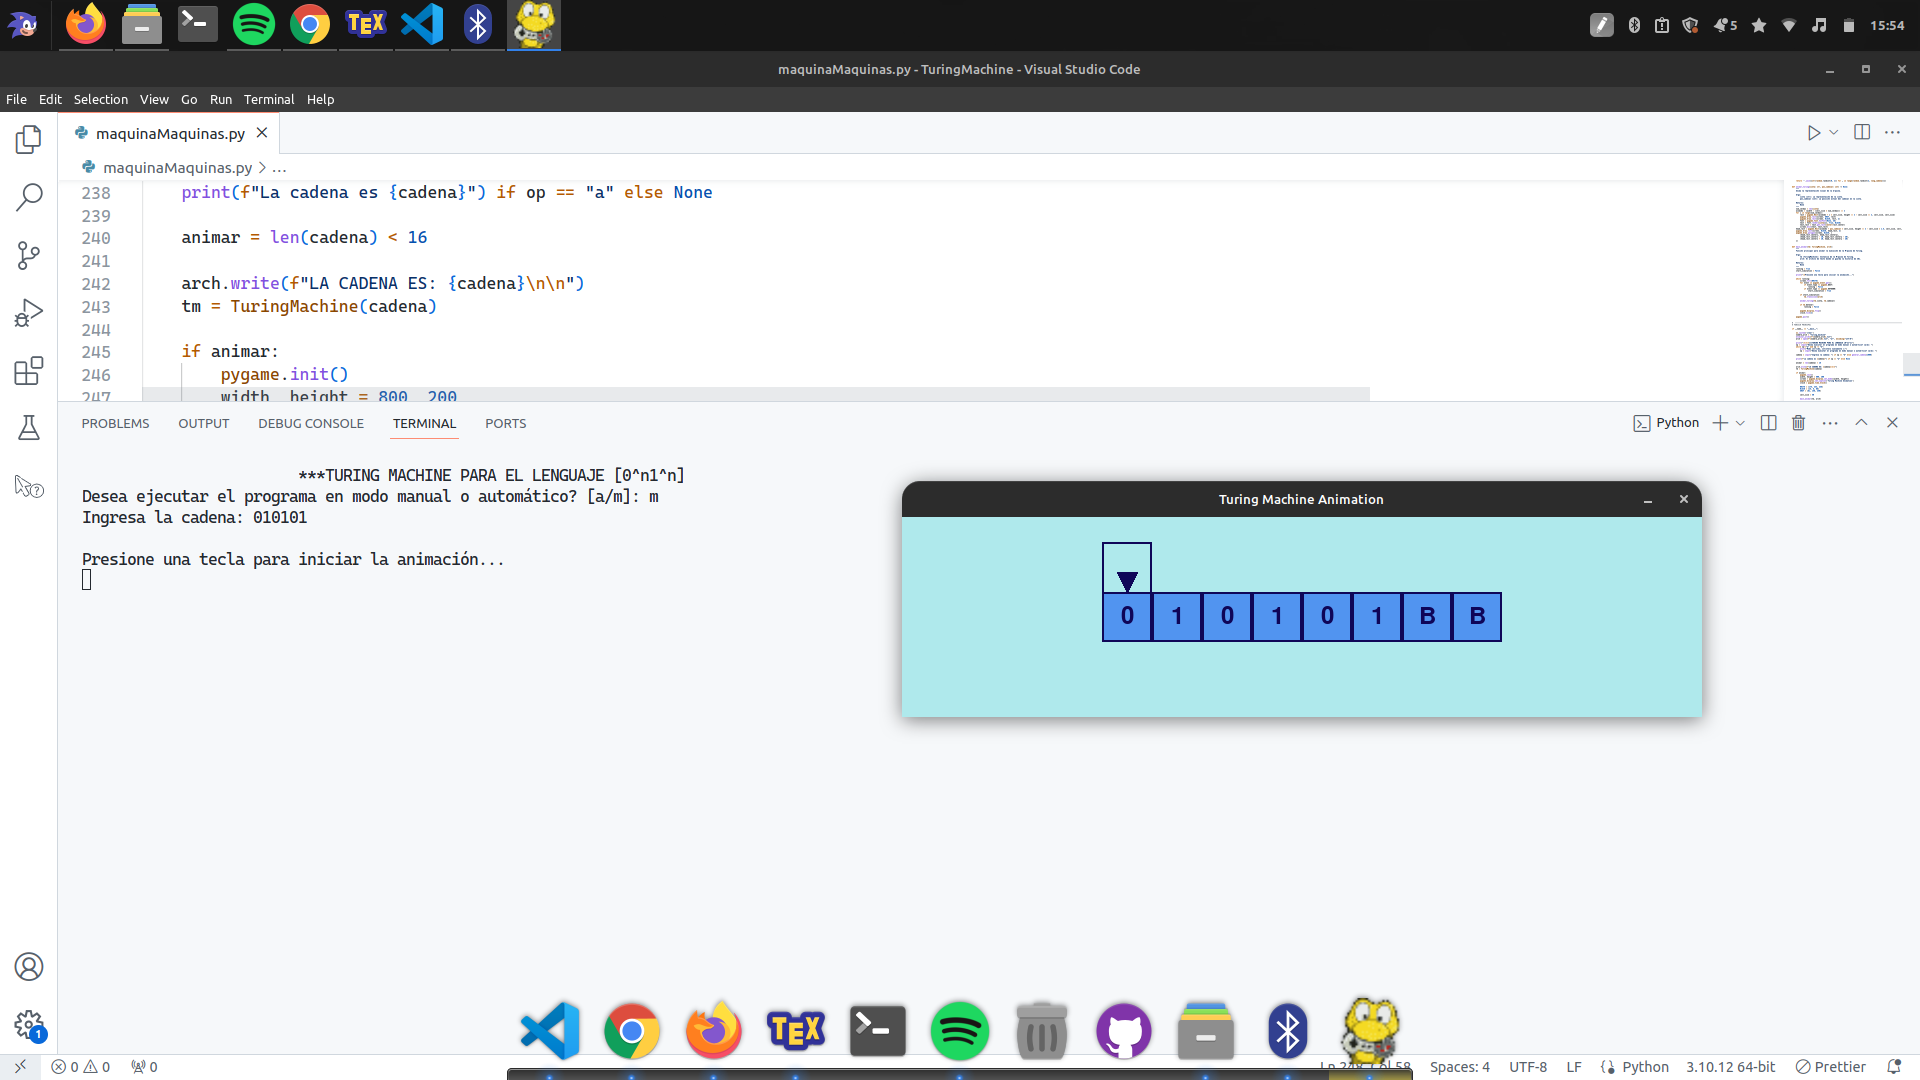
\includegraphics[width=0.8\textwidth]{manual5}
		\caption{Cadena 010101 - Animación de la Máquina de Turing}
	\end{figure}
	
	\newpage
	\begin{figure}[h]
		\centering
		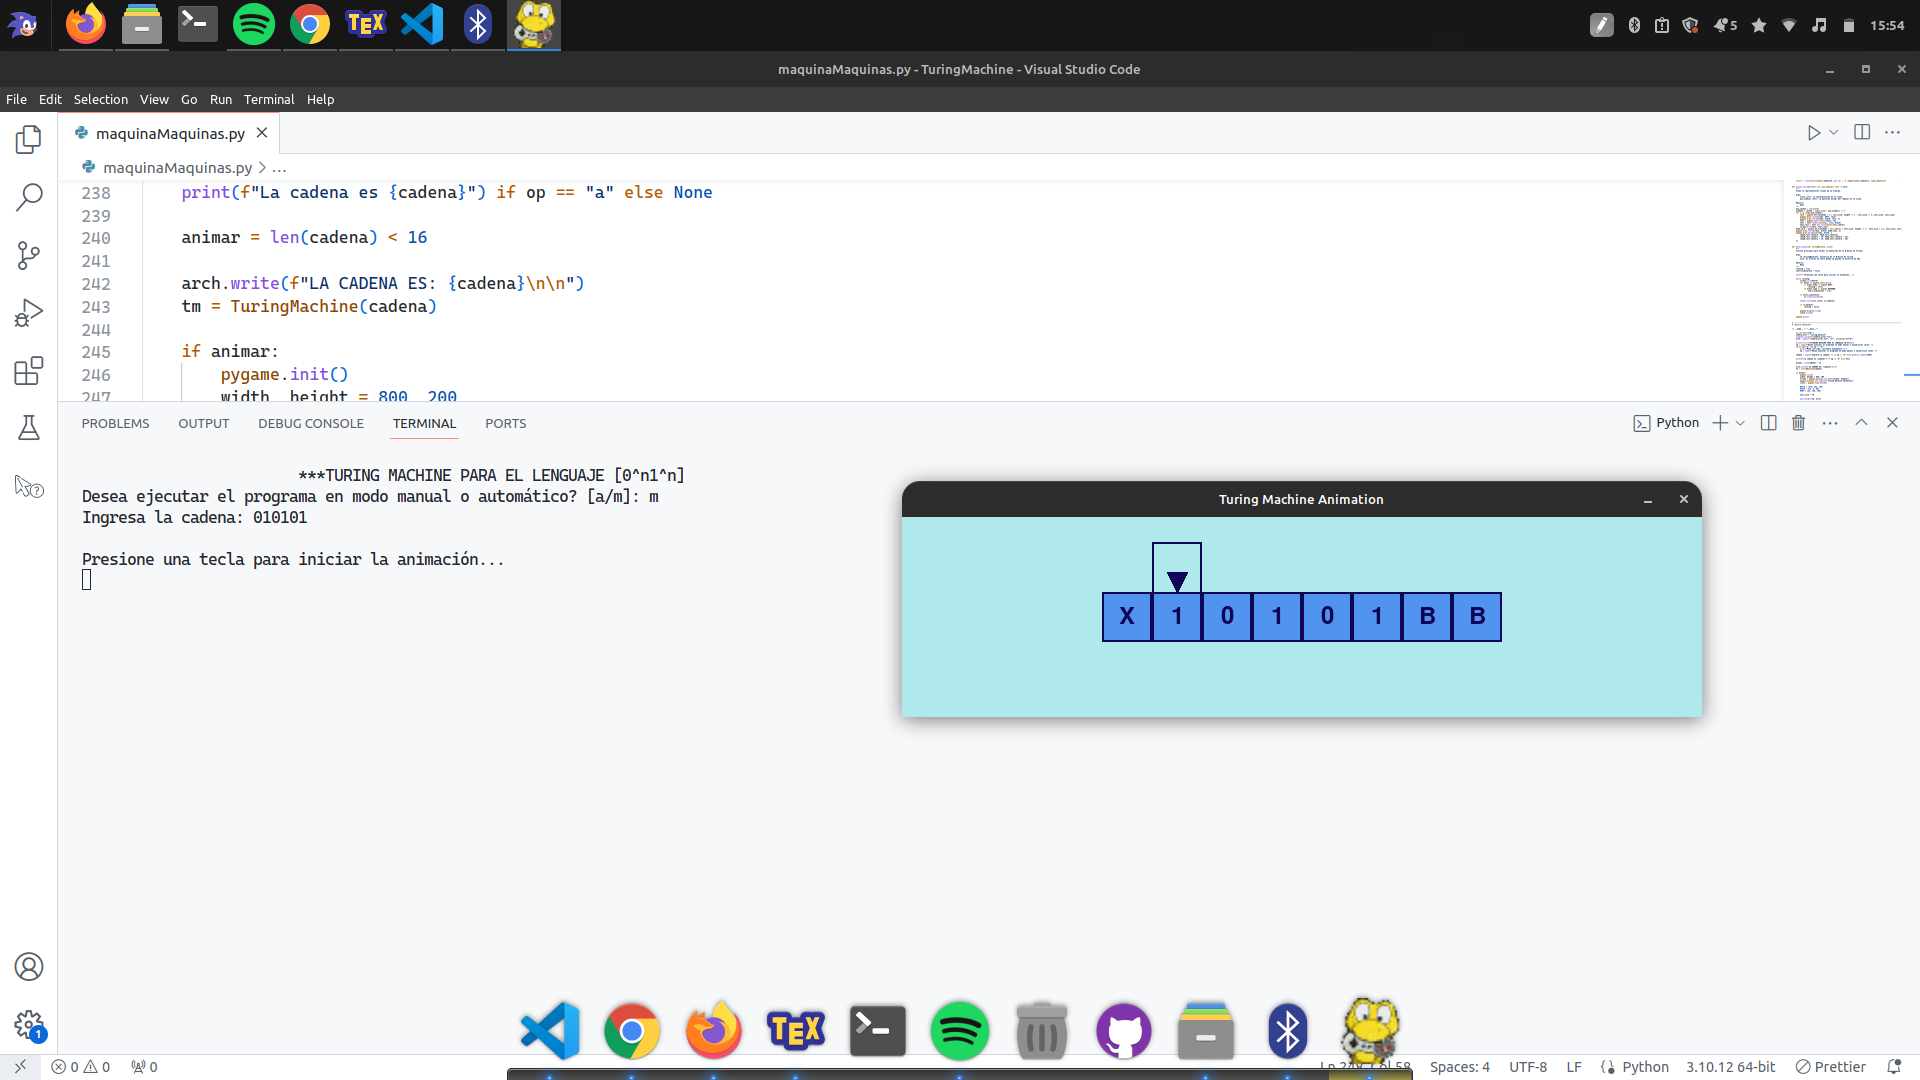
\includegraphics[width=0.8\textwidth]{manual6}
		\caption{Cadena 010101 - Animación de la Máquina de Turing}
	\end{figure}
	\begin{figure}[h]
		\centering
		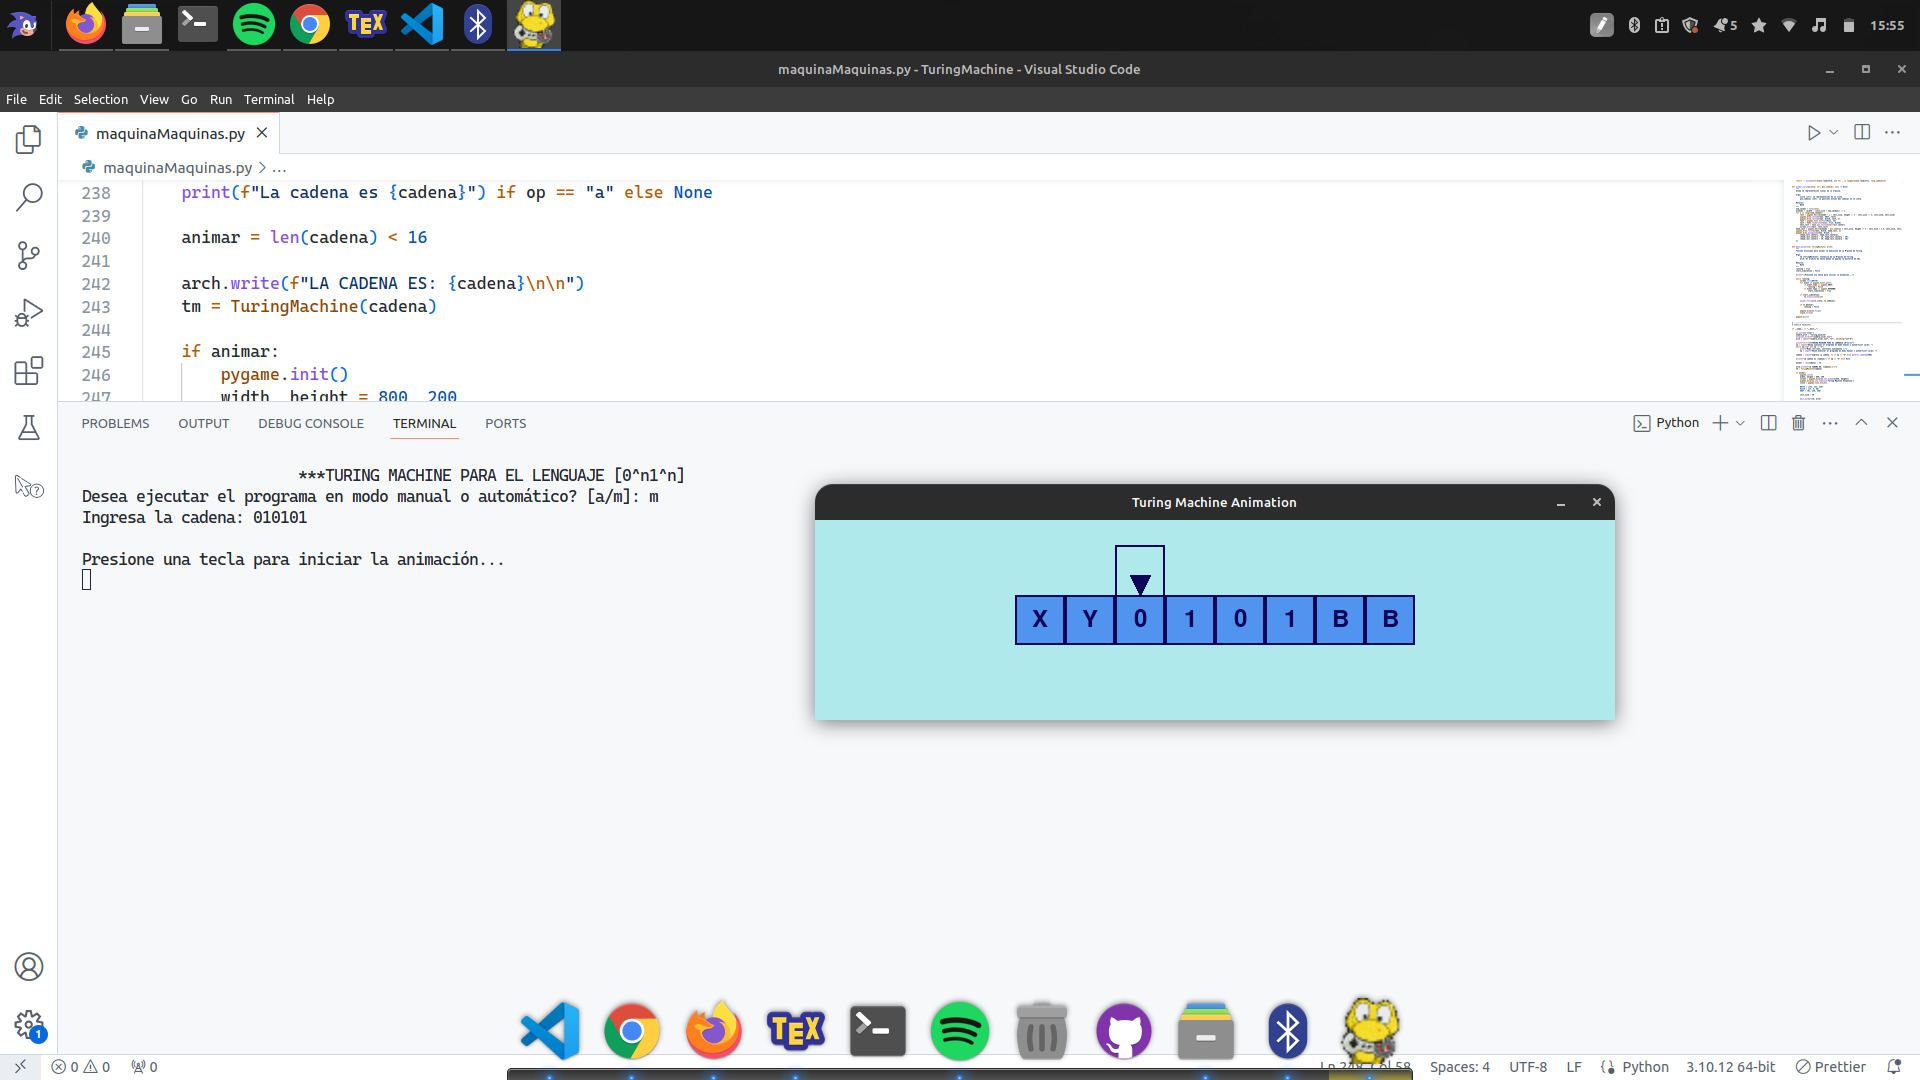
\includegraphics[width=0.8\textwidth]{manual7}
		\caption{Cadena 010101 - Animación de la Máquina de Turing}
	\end{figure}
	
	\newpage	
	\begin{figure}[h]
		\centering
		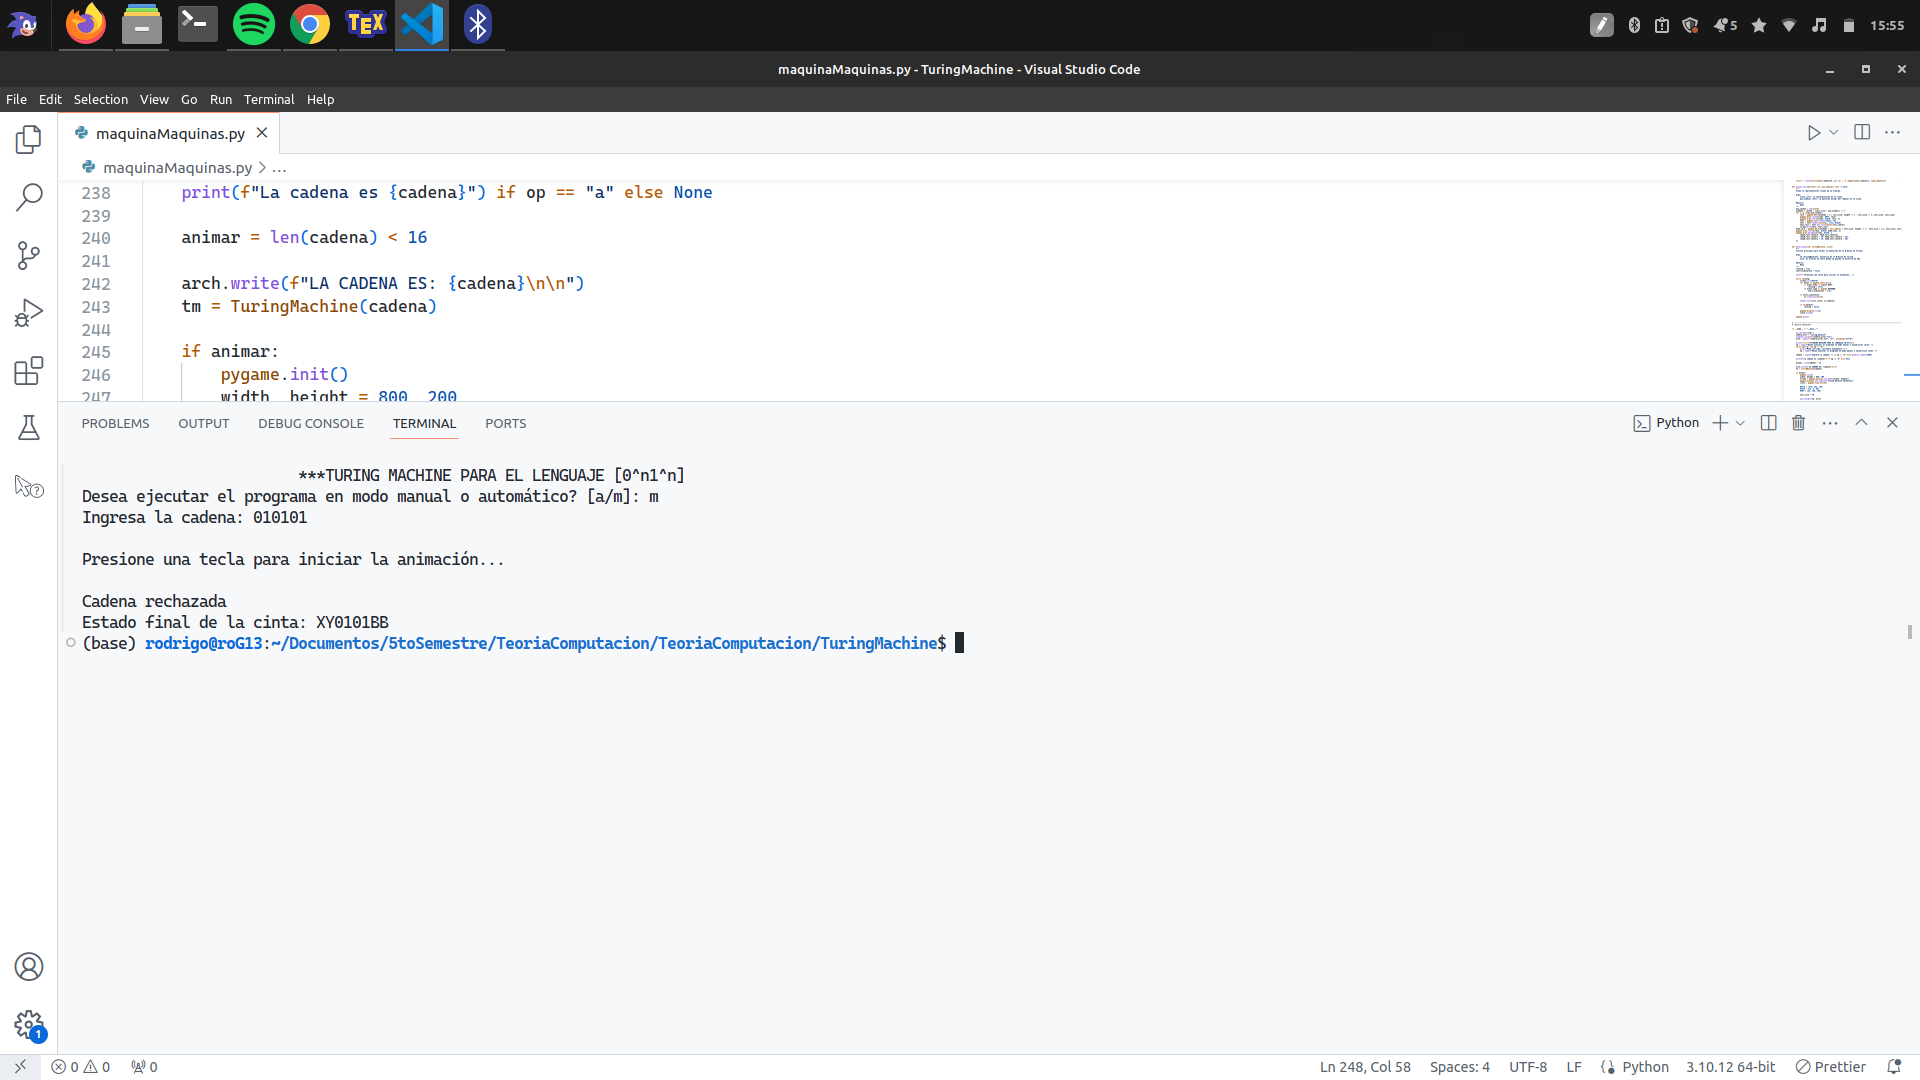
\includegraphics[width=0.8\textwidth]{manual8}
		\caption{Cadena 010101 - Resultados}
	\end{figure}
	\begin{figure}[h]
		\centering
		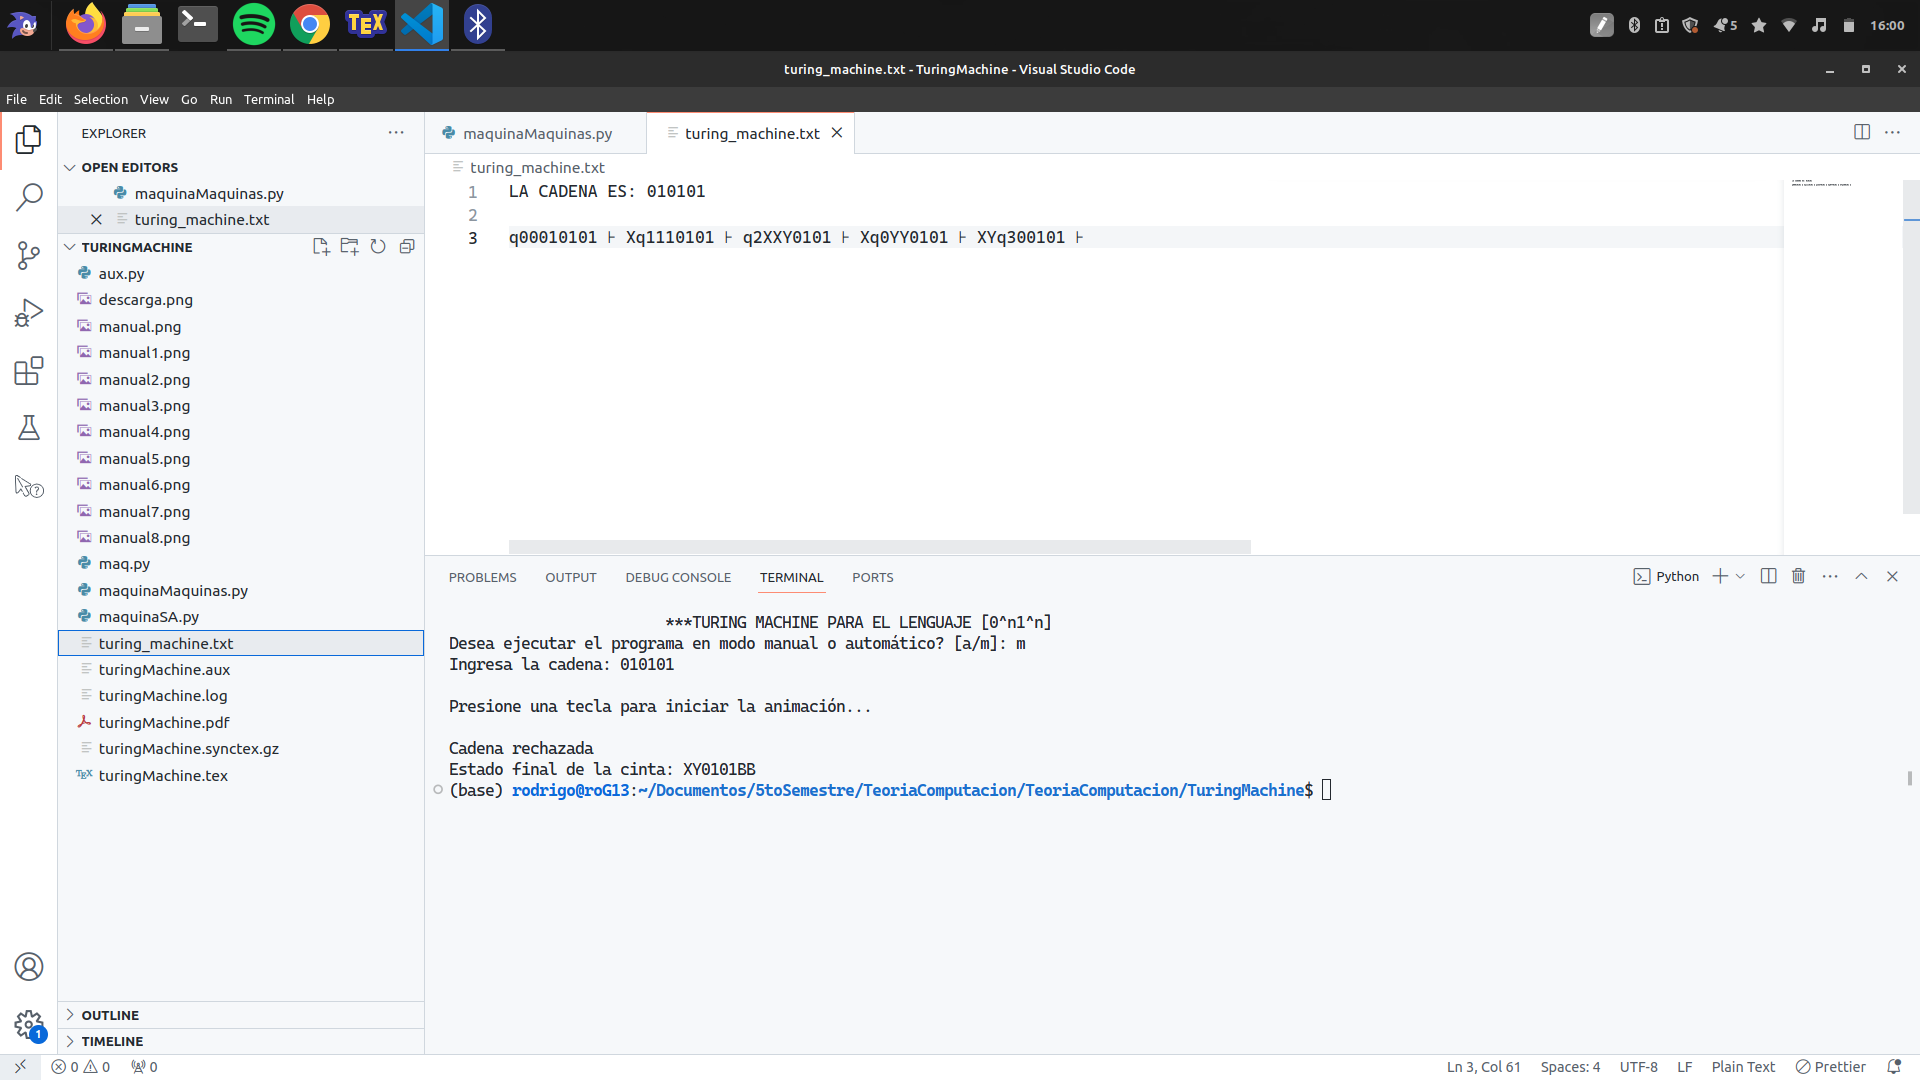
\includegraphics[width=0.8\textwidth]{arch2}
		\caption{Cadena 010101 - Archivo de los ID's}
	\end{figure}
	
	\newpage
		\begin{figure}[h]
		\centering
		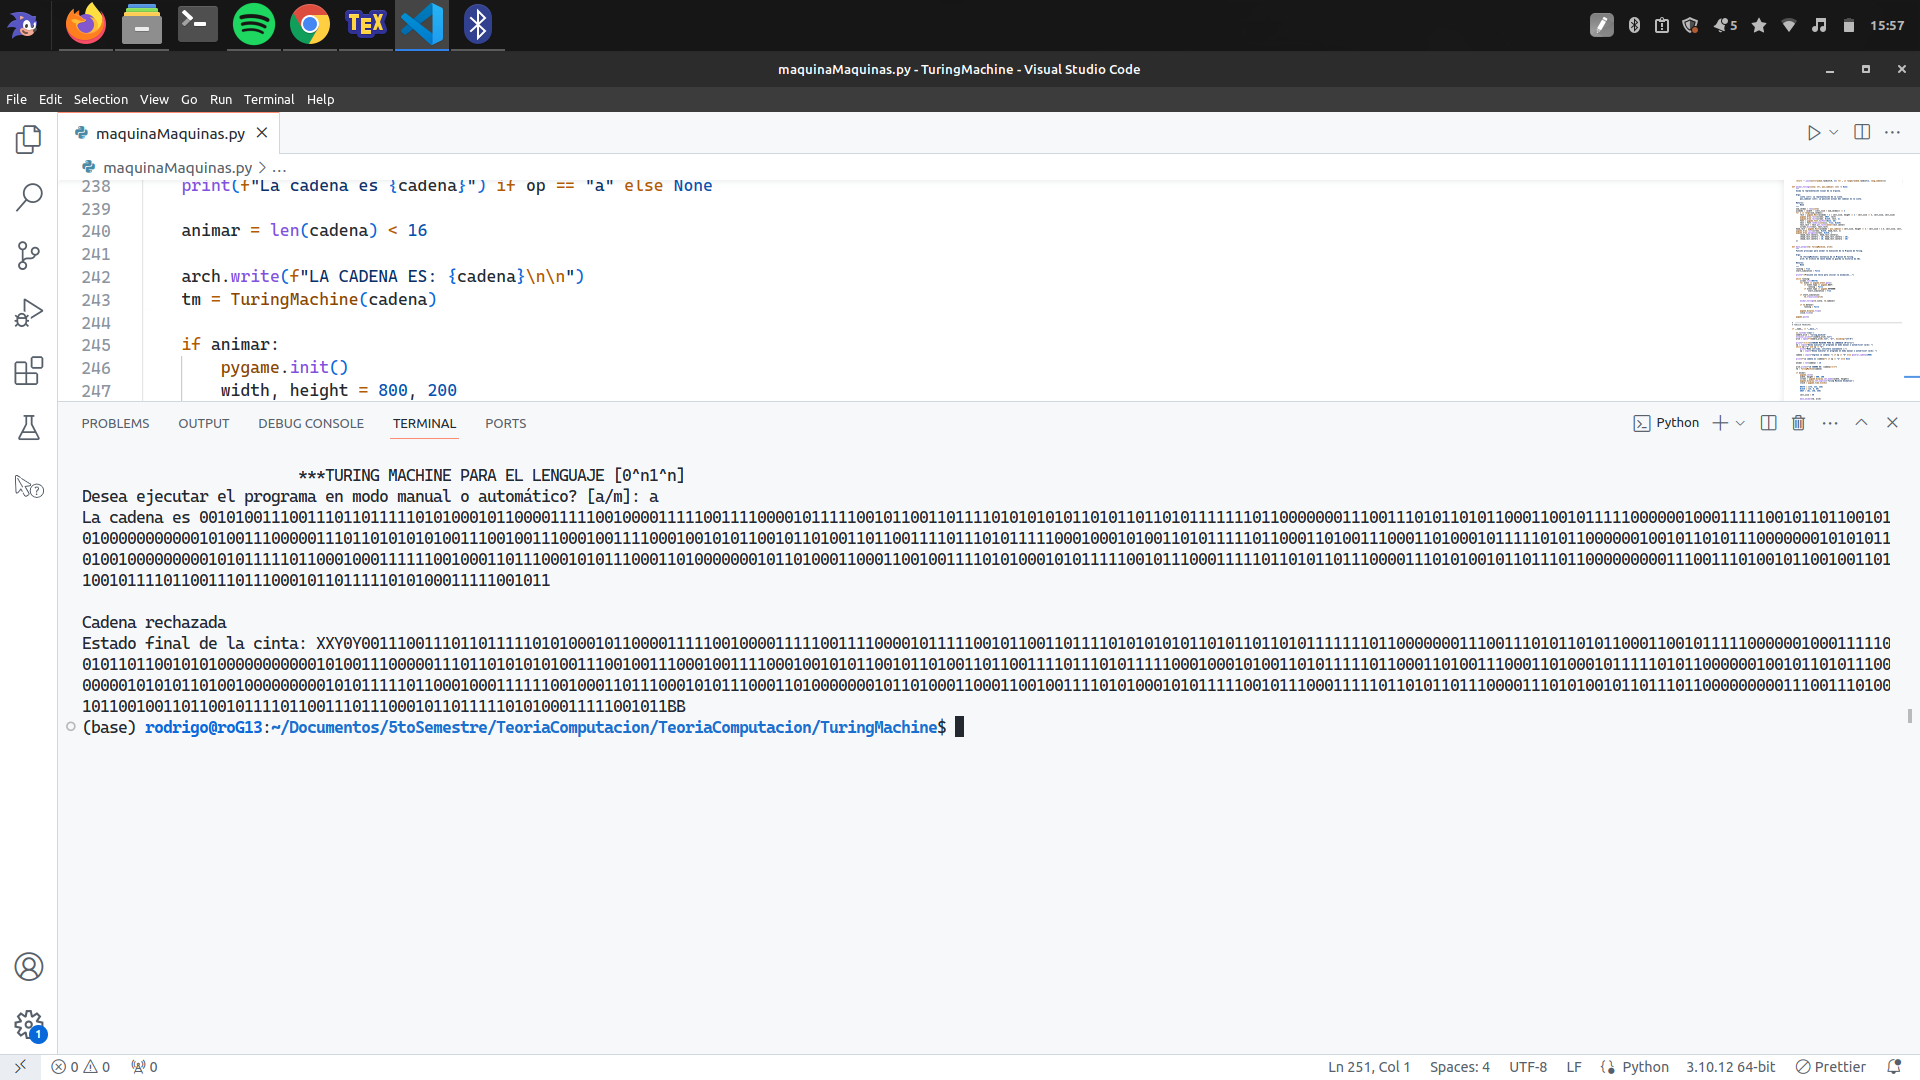
\includegraphics[width=0.8\textwidth]{auto}
		\caption{Modo automático}
	\end{figure}
	\begin{figure}[h]
		\centering
		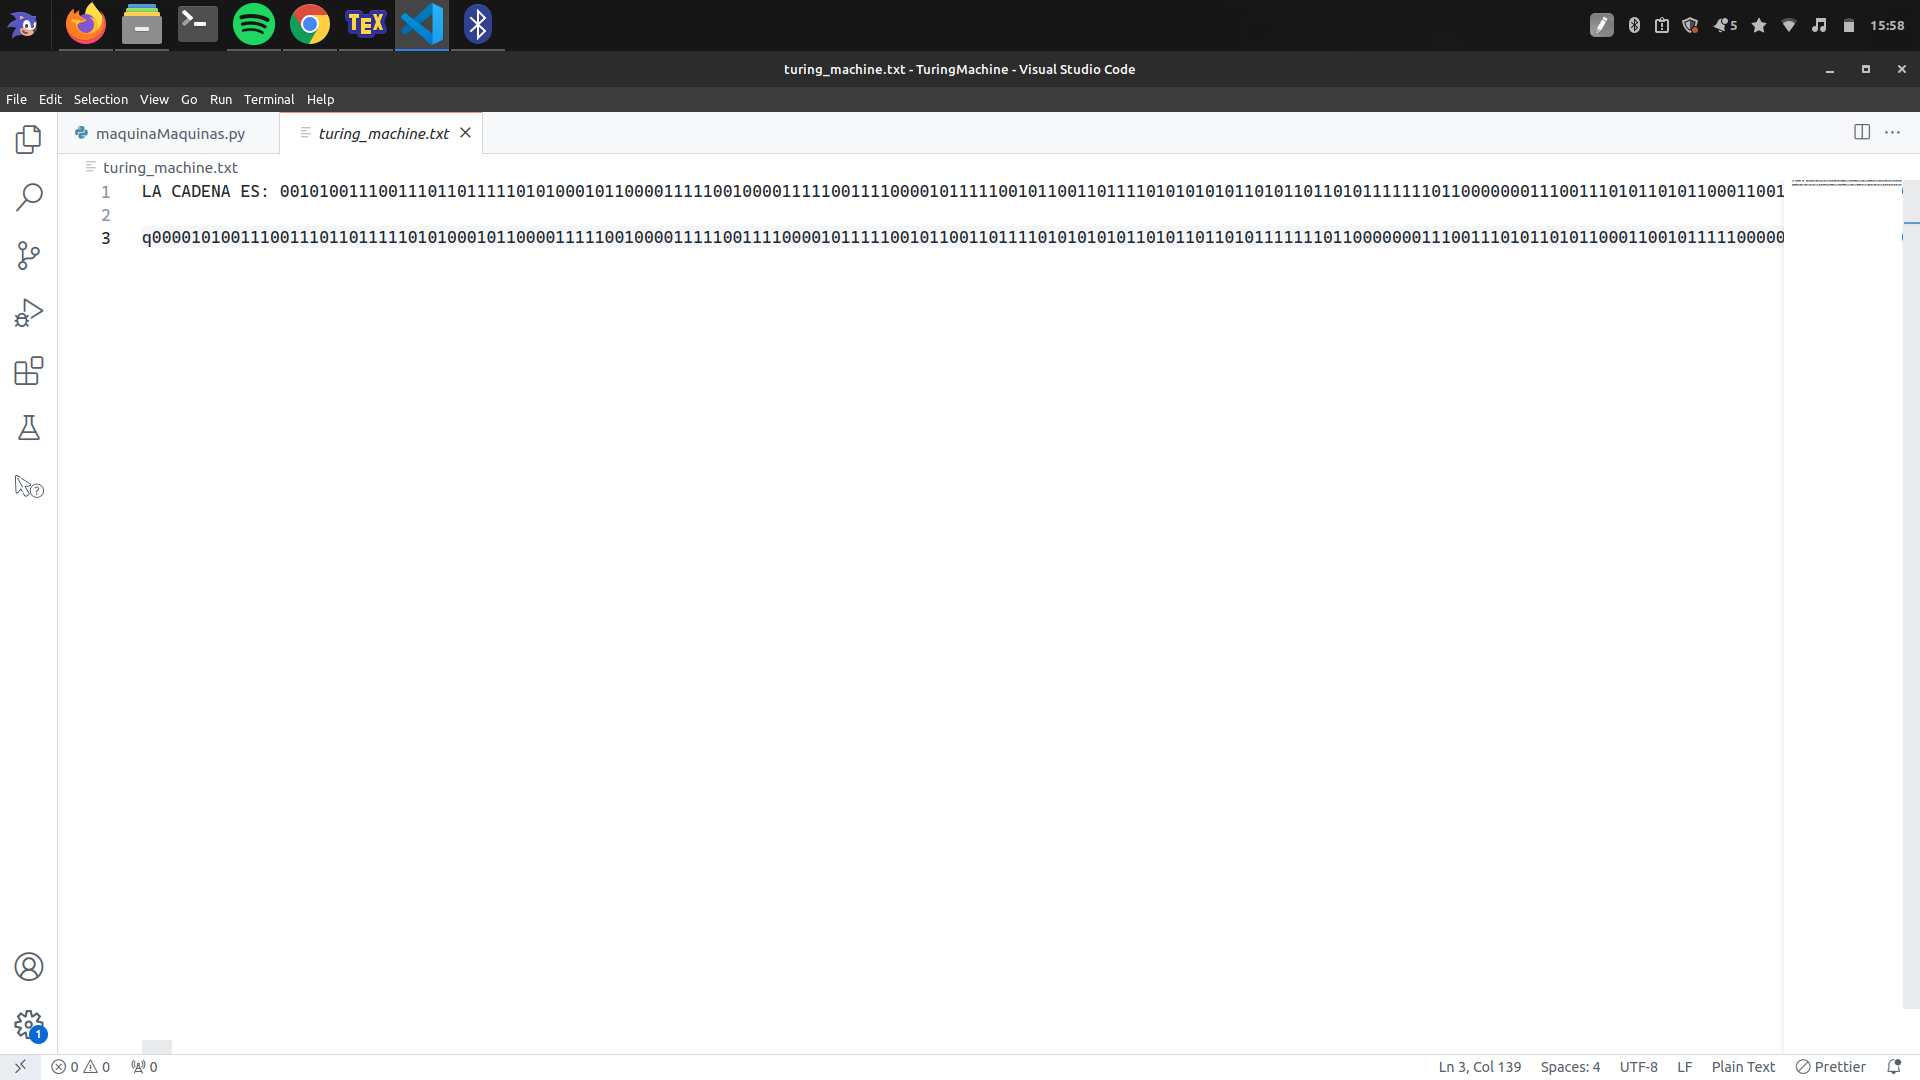
\includegraphics[width=0.8\textwidth]{arch3}
		\caption{Modo automático - Archivo de ID's}
	\end{figure}
	

	
	
	
	\newpage
	\section*{Conclusión}
	
	En esta práctica, he explorado y desarrollado una Máquina de Turing capaz de reconocer el lenguaje \( \{0^n1^n | n \geq 1\} \), un lenguaje clásico en la teoría de la computación que requiere un equilibrio preciso entre ceros y unos. A través de la implementación de la tabla de transiciones proporcionada y las pruebas realizadas con diversas cadenas de entrada, se ha demostrado la capacidad de la Máquina de Turing para determinar la aceptación de cadenas válidas dentro del lenguaje.
	
	La práctica me permitió profundizar en el funcionamiento interno de las Máquinas de Turing, desde la definición de estados y transiciones hasta la visualización del procesamiento de la cinta en tiempo real. A pesar de su simplicidad conceptual, la Máquina de Turing que se ha construido ilustra la potencia del modelo de Turing para la computación y cómo incluso las máquinas más simples pueden realizar tareas de reconocimiento de patrones complejos.
	
	Es así que, esta experiencia ha reforzado mi entendimiento de los conceptos teóricos subyacentes a las Máquinas de Turing y ha me proporcionado una base sólida para futuros estudios en el campo de la teoría de la computación y la ciencia de la computación en general.
	
		
	\section*{Bibliografía}
	
	
	[1] “Turing Machine in TOC - GeeksforGeeks”. GeeksforGeeks. Accedido el 25 de diciembre de 2023. [En línea]. Disponible: https://www.geeksforgeeks.org/turing-machine-in-toc/
	
	
	[2] “Definición de máquina de Turing y ejemplos – BorrowBits”. BorrowBits. Accedido el 25 de diciembre de 2023. [En línea]. Disponible: https://borrowbits.com/2013/03/maquinas-de-turing/
	
	[3] J. Ullman. “CS154: Introduction to automata and complexity theory”. The Stanford University InfoLab. Accedido el 25 de diciembre de 2023. [En línea]. Disponible: http://infolab.stanford.edu/\~{}ullman/ialc/
	spr10/spr10.html\#LECTURE\%20NOTES
	
	
	\newpage
	\section{Anexo - Código de Implementación}
	
	\begin{lstlisting}
	
	'''
	INSTITUTO POLITECNICO NACIONAL
	ESCUELA SUPERIOR DE COMPUTO
	
	INGENIERIA EN INTELIGENCIA ARTIFICIAL
	
	TEORIA DE LA COMPUTACION
	MAQUINA DE TURING
	
	GRUPO: 5BM1
	ALUMNO: TREJO ARRIAGA RODRIGO GERARDO
	
	ESTE PROGRAMA GENERA UNA MAQUINA DE TURING QUE VALIDA SI UNA CADENA PERTENECE AL LENGUAJE 0^n1^n Y:
	i) SOLICITA AL USUARIO UNA CADENA A VALIDAR O LA GENERA DE MANERA RANDOM
	ii) ANIMA LA MAQUINA DE TURING SI LA LONGITUD DE LA PALABRA ES MENOR A 16
	iii) GENERA LA HISTORIA DE ID's EN UN ARCHIVO DE TEXTO
	
	ULTIMA MODIFICACION: 25/12/2023
	'''
	
	#  ------------------------------------------------
	# MODULOS Y LIBRERIAS IMPORTADAS
	
	import pygame
	import os
	import random
	
	#  ------------------------------------------------
	# CLASES
	
	
	class TuringMachine:
	
		def __init__(self, cinta_string: str, simbolo_blanco: str ="B") -> None:
			"""
			Inicializa la Maquina de Turing.
			
			Args:
			cinta_string (str): La cadena de entrada para la maquina.
			simbolo_blanco (str): El simbolo que representa un espacio en blanco en la cinta.
			"""
			self.cinta = list(cinta_string) + [simbolo_blanco] * 2
			self.cabezal = 0
			self.estado = 'q0'
			self.simbolo_blanco = simbolo_blanco
			self.detener = False
			self.tabla_trans = {
				('q0', '0'): ('q1', 'X', 'R'),
				('q0', 'Y'): ('q3', 'Y', 'R'),
				('q1', '0'): ('q1', '0', 'R'),
				('q1', '1'): ('q2', 'Y', 'L'),
				('q1', 'Y'): ('q1', 'Y', 'R'),
				('q2', '0'): ('q2', '0', 'L'),
				('q2', 'X'): ('q0', 'X', 'R'),
				('q2', 'Y'): ('q2', 'Y', 'L'),
				('q3', 'Y'): ('q3', 'Y', 'R'),
				('q3', self.simbolo_blanco): ('q4', self.simbolo_blanco, 'R'),
			}
		
		
		def es_aceptada(self) -> bool:
			"""
			Verifica si la maquina de Turing ha llegado a un estado de aceptacion.
			
			Returns:
			bool: True si esta en un estado de aceptacion, False de lo contrario.
			"""
			return self.estado == 'q4'
		
		
		def es_rechazada(self) -> bool:
			"""
			Verifica si la maquina de Turing ha llegado a un estado de rechazo.
			
			Returns:
			bool: True si esta en un estado de rechazo, False de lo contrario.
			"""
			return self.estado != 'q4'
		
		
		def transicion(self, arch) -> None:
			"""
			Realiza una transicion de la maquina de Turing.
			
			Args:
			arch: El archivo de texto donde se guarda la historia de IDs.
			"""
			if self.detener:
			return None
			
			simbolo_act = self.cinta[self.cabezal]
			
			alfa = ''.join(self.cinta[:self.cabezal]).replace("B", "")
			q = self.estado
			beta = ''.join(self.cinta[self.cabezal:]).replace("B", "")
			arch.write(f"{alfa}{q}{simbolo_act if simbolo_act != 'B' else ''}{beta} -> ")
			
			accion = self.tabla_trans.get((self.estado, simbolo_act))
			
			if accion is None:
			self.detener = True
			else:
			nuevo_estado, nuevo_simbolo, direccion = accion
			self.cinta[self.cabezal] = nuevo_simbolo
			self.cabezal += 1 if direccion == 'R' else -1
			self.estado = nuevo_estado
		
		
		def run(self, arch) -> bool:
			"""
			Ejecuta la Maquina de Turing hasta que se detiene.
			
			Args:
			arch: El archivo de texto donde se guarda la historia de IDs.
			
			Returns:
			bool: True si la cadena fue aceptada, False de lo contrario.
			"""
			while not self.detener:
			self.transicion(arch)
			
			return self.estado == 'q4'
	
	
	#  -------------------------------------------------
	
	# FUNCIONES
	
	
	def eliminar_archs(nombre_arch: str) -> None:
		"""Funcion que elimina un archivo si existe en el directorio
		
		Args:
		nombre_arch (str): Nombre del archivo que deseas eliminar
		"""
		archivo1 = nombre_arch
		if os.path.exists(archivo1):
		os.remove(archivo1)
	
	
	def generar_cadena(long_cadena:int) -> str:
		"""Funcion que genera la cadena binaria random
		
		Args:
		long_cadena (int): Longitud de la palabra binaria
		
		Returns:
		str: Palabra binarias
		"""
		return ''.join([str(random.randint(0, 1)) for _ in range(random.randint(2, long_cadena))])
	
	
	def animar_turing(cinta: str, pos_cabezal: int) -> None:
		"""
		Anima la representacion visual de la maquina.
		
		Args:
		cinta (str): La representacion de la cinta.
		pos_cabezal (int): La posicion actual del cabezal en la cinta.
		
		Returns:
		None
		"""
		num_celdas = len(cinta)
		acomodo = (width - (cell_size * num_celdas)) // 2
		for i in range(num_celdas):
		rect = pygame.Rect(acomodo + i * cell_size, height // 2 - cell_size // 2, cell_size, cell_size)
		pygame.draw.rect(screen, GRAY, rect)
		pygame.draw.rect(screen, BLACK, rect, 2)
		font = pygame.font.SysFont(None, 36)
		text = font.render(cinta[i], True, BLACK)
		text_rect = text.get_rect(center=rect.center)
		screen.blit(text, text_rect)
		head_rect = pygame.Rect(acomodo + pos_cabezal * cell_size, height // 2 - cell_size * 1.5, cell_size, cell_size * 2)
		pygame.draw.rect(screen, BLACK, head_rect, 2)
		pygame.draw.polygon(screen, BLACK, [
		(head_rect.centerx, head_rect.centery),
		(head_rect.centerx - 10, head_rect.centery - 20),
		(head_rect.centerx + 10, head_rect.centery - 20)
		])
	
	
	def main_animar(tm: TuringMachine, arch):
		"""
		Funcion principal para animar la ejecucion de la Maquina de Turing.
		
		Args:
		tm (TuringMachine): Instancia de la Maquina de Turing.
		arch: El archivo de texto donde se guarda la historia de IDs.
		
		Returns:
		None
		"""
		running = True
		start_simulation = False
		
		while running:
		screen.fill(WHITE)
		for event in pygame.event.get():
		if event.type == pygame.QUIT:
		running = False
		if event.type == pygame.KEYDOWN:
		start_simulation = True
		
		if start_simulation:
		tm.transicion(arch)
		
		animar_turing(tm.cinta, tm.cabezal)
		
		if tm.detener:
		running = False
		
		pygame.display.flip()
		clock.tick(1)
		
		pygame.quit()
	
	
	#  -----------------------------------------------------
	
	# FUNCION PRINCIPAL 
	
	if __name__ == "__main__":
	
		os.system('clear')
		nombre_arch = "turing_machine"
		eliminar_archs(f"{nombre_arch}.txt")
		arch = open(f"{nombre_arch}.txt", "a+", encoding="utf-8")
		
		print("\t\t\t***TURING MACHINE PARA EL LENGUAJE [0^n1^n]")
		op = input("Desea ejecutar el programa en modo manual o automatico? [a/m]: ")
		while op!="a" and op != "m":
		print("Modo invalido, intentelo nuevamente ):")
		op = input("Desea ejecutar el programa en modo manual o automatico? [a/m]: ")
		
		cadena = input("Ingresa la cadena: ") if op == "m" else generar_cadena(1000)
		
		print(f"La cadena es {cadena}") if op == "a" else None
		
		animar = len(cadena) < 16
		
		arch.write(f"LA CADENA ES: {cadena}\n\n")
		tm = TuringMachine(cadena)
		
		if animar:
			pygame.init()
			width, height = 800, 200
			screen = pygame.display.set_mode((width, height))
			pygame.display.set_caption('Turing Machine Animation')
			clock = pygame.time.Clock()
			
			WHITE = (175, 233, 236)
			BLACK = (15, 6, 88)
			GRAY = (81, 148, 240)
			
			cell_size = 50
			
			main_animar(tm, arch)
		
		else:
			is_accepted = tm.run(arch)
		
		if tm.es_aceptada():
			print("Cadena aceptada")
		elif tm.es_rechazada():
			print("Cadena rechazada")
		else:
			print("Detenida!!!")
		
		print(f"Estado final de la cinta: {''.join(tm.cinta)}")
		arch.close()
		
	
	
	\end{lstlisting}

	
	
\end{document}